\documentclass[a4paper,12pt]{article}
\usepackage[indonesian]{babel}
\usepackage{graphicx}
\usepackage{multirow}
\usepackage{enumitem}
\usepackage{listings}
\usepackage{wrapfig}
\usepackage[T1]{fontenc}
\usepackage{inconsolata}
\usepackage{lipsum}
\usepackage{adjustbox}


\usepackage{color}
\usepackage[table]{xcolor}
\definecolor{mygreen}{rgb}{0,0.6,0}
\definecolor{mygray}{rgb}{0.5,0.5,0.5}
\definecolor{mymauve}{rgb}{0.58,0,0.82}
\lstset{%
    language=java,
    showstringspaces=false,          % Prevent tex replacing space to bracket in code
    frame=single,                    % Set frame around code
    backgroundcolor=\color{white},   % choose the background color
    basicstyle=\footnotesize,        % size of fonts used for the code
    breaklines=true,                 % automatic line breaking only at whitespace
    captionpos=b,                    % sets the caption-position to bottom
    commentstyle=\color{mygreen},    % comment style
    keywordstyle=\color{blue},       % keyword style
    stringstyle=\color{mymauve},     % string literal style
}

\graphicspath{ {./img/} }
\begin{document}
\title{ {\Large Laporan Praktikum}\\ Algoritma dan Pemrograman Lanjut\\{\Large Pertemuan 8}}

\author{Aldzikri Dwijayanto Prathama
    \\195410189
    \\Informatika}
\makeatletter
\begin{titlepage}
    \begin{center}
        {\huge \bfseries \@title}\\[14ex]
        
\includegraphics[scale=.8]{logo}\\[4ex]
        {\large \@author}\\[12ex]
        {\large \bfseries {SEKOLAH TINGGI MANAJEMEN INFORMATIKA DAN KOMPUTER
            AKAKOM YOGYAKARTA}}
    \end{center}


%{\large \@date}
\end{titlepage}
\makeatother
%\maketitle
\newpage
\tableofcontents
\newpage

\section{Tujuan}
Mahasiswa dapat memahami, membuat dan menyelesaikan kasus dengan
menggunakan method tanpa parameter

\section{Teori}
\paragraph{}
Fungsi digunakan untuk mempermudah didalam membuat sebuah program, terutama
program yang besar dan banyak melakukan beberapa hal yang sama. Fungsi memiliki ciri-ciri
sebagai berikut:
\begin{enumerate}
    \item Memiliki nama dari fungsi tersebut.
    \item Memiliki tugas spesifik tertentu.
    \item Memiliki sekumpulan statement atau perintah untuk melakukan tugas tersebut.
    \item Mengembalikan sebuah nilai kepada fungsi lain yang memanggil atau menggunakannya (jika perlu).
\end{enumerate}
\newpage

\section{Pembahasan}
\subsection{Praktik}
\subsubsection{Praktik 1}
\textbf{Menggunakan method tanpa parameter}
\begin{lstlisting}
public class method1{
	public static void cetak(){
		System.out.println("STIMIK AKAKOM");
	}
	public static void main(String args []){
		cetak();
	}
}
\end{lstlisting}
Method diatas bersifat static dan bertipe void sehingga tidak mengembalikan nilai, dan hanya akan menampilkan tulisan
STMIK AKAKOM ke layar. Method yang bersifat static bisa langsung dipanggil dengan nama methodnya saja.Sebuah method juga
bisa dipanggil lebih dari satu kali.\\

Jika program dijalankan, maka hasilnya seperti berikut:
\begin{center}
    
\includegraphics{1.png} 
\end{center}

\subsubsection{Praktik 2}
\textbf{Pemanggilan method lebih dari sekali}
\begin{lstlisting}
public class method2{
	public static void cetakkalimat(){
		System.out.println("didalam method kalimat");
	}
	public static void main(String args []){
		cetakkalimat();
		System.out.println("di dalam main");
		cetakkalimat();
	}
}
\end{lstlisting}

Method diatas bersifat static dan bertipe void sehingga tidak mengembalikan nilai, method tersebut hanya akan menampilkan tulisan
``didalam method kalimat'' ke layar. Method yang bersifat static bisa langsung dipanggil dengan nama methodnya saja. Sebuah method juga
bisa dipanggil lebih dari satu kali. Pada bagian program main, terlihat method tersebut di panggil sebanyak dua kali.

Jika program dijalankan, maka hasilnya seperti berikut:
\begin{center}
    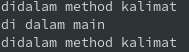
\includegraphics{2.png} 
\end{center}

\subsubsection{Praktik 3}
\textbf{Menggunakan method dalam perulangan}
\begin{lstlisting}
public class method3{
	public static void cetak(){
		System.out.println("STIMIK AKAKOM");
	}
	public static void main(String args []){
		for (int i=0;i<10; i++)
		cetak();
	}
}
\end{lstlisting}
Karena method dapat dipanggil lebih dari satu kali, maka method juga dapat dipanggil dengan perulangan di dalam program
main.

Jika program dijalankan, maka hasilnya seperti berikut:
\begin{center}
    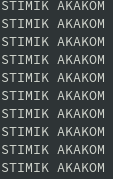
\includegraphics{3.png} 
\end{center}

\subsubsection{Praktik 4}
\textbf{Method tanpa parameter dengan nilai balik (return type)}
\begin{lstlisting}
public class method4{
	public static int jumlah(){
		int a=8 ,b=10;
		return (a+b);
	}
	public static void main(String args []){
		System.out.println("hasil pemangilan method jumlah");
		System.out.println(jumlah());
	}
}
\end{lstlisting}
Method diatas merupakan method non void, yang berarti method tersebut akan mengembalikan atau menghasilkan nilai. Karena
method memiliki return type integer, itu berarti nilai yang dikembalikan atau dihasilkan memiliki tipe data integer.
Peryataan terkahir dari method tersebut adalah return, penyataan ini wajib diberikan untuk method non void, yang
menginstruksikan program untuk mengembalikan nilai ke nama fungsi.

Jika program dijalankan, maka hasilnya seperti berikut:
\begin{center}
    
\includegraphics{4.png} 
\end{center}

\subsubsection{Praktik 5}
\textbf{Memanggil method dengan menciptakan objek}
\begin{lstlisting}
public class method5{
	public static int jumlah(){
		int a=8 ,b=10;
		return (a+b);
	}
	public static void main(String args []){
		method5 obyek=new method5();
		System.out.println("hasil pemangilan method jumlah");
		System.out.println(obyek.jumlah());
	}
}
\end{lstlisting}
Pada program di atas terdapat method non-void, yang akan mengembalikan nilai dalam bentuk integer. Pada program main,
dibuat objek baru, yaitu obyek.jumlah, sehingga untuk memanggil method dengan objek adalah dengan memanggil
obyek.jumlah.

Jika program dijalankan, maka hasilnya seperti berikut:
\begin{center}
    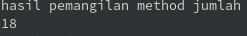
\includegraphics{5.png} 
\end{center}

\newpage

\subsection{Latihan}
Program dengan menggunakan method untuk menampilkan data pribadi Anda seperti NIK, Nama, Jenis kelamin, Umur, Alamat.
\begin{lstlisting}
public class Latihan1 {
	public static void data(){
		System.out.println("NIK\t\t: 123**************");
		System.out.println("Nama\t\t: Aldzikri Dwijayanto Prathama");
		System.out.println("Jenis Kelamin\t: Laki-laki");
		System.out.println("Umur\t\t: 18");
		System.out.println("Alamat\t\t: Klaten Tengah, Klaten, Jawa Tengah");
		}
		public static void main(String args[]){
			data();
		}
}
\end{lstlisting}
Pada program latihan tersebut terdapat method, yang di dalamnya terdapat pernyataan yang akan menampilkan data pribadi,
kemudian method tersebut dipanggil pada program main.

Jika program dijalankan, maka hasilnya seperti berikut:
\begin{center}
    
\includegraphics{6.png} 
\end{center}

\newpage

\section{Kesimpulan}
Setelah praktik mahasiswa dapat memahami, membuat dan menyelesaikan kasus dengan
menggunakan method tanpa parameter

\end{document}
